\documentclass[10pt]{article}
 
\usepackage[margin=1in]{geometry} 
\usepackage{amsmath,amsthm,amssymb, graphicx, multicol, array}
 
\newcommand{\N}{\mathbb{N}}
\newcommand{\Z}{\mathbb{Z}}
 
\newenvironment{problem}[2][Problem]{\begin{trivlist}
\item[\hskip \labelsep {\bfseries #1}\hskip \labelsep {\bfseries #2.}]}{\end{trivlist}}

\begin{document}
 
\title{M. Krumholz: Notes on Star Formation (2018)}
\author{Sean Lewis\\
Problem Set : Summer 2019}
\maketitle
 
\begin{problem}{1.1}
\textbf{Molecular Tracers.}\\
Here we will derive a definition of the critical density, and use it to compute some critical densities for important molecular transitions. For the purposes of this problem, you will need to know some basic parameters (such as energy levels and Einstein coefficients) of common interstellar molecules. You can obtain these from http://www.strw.leidenuniv.nl/~moldata . It is also worth taking a quick look through the associated paper (Schoier et al., 2005) so you get a feel for where these numbers come from.
\end{problem}
\textbf{(a).} Consider an excited state $i$ of some molecule, and let $A_{ij}$ and $k_{ij}$ be the Einstein A coefficient and the collision rate, respectively, for transitions from state $i$ to state $j$. Write down expressions for the rates of spontaneous radiative and collisional de-excitations out of state $i$ in a gas where the number density of collision partners is $n$.

\begin{proof}[Solution]
The radiative de-excitation rate (the rate of spontaneous emission) is obviously dependent on the de-excitation rate from the excited to de-excited state $A_{ij}$ and the density of atoms that are in the exited state $i$. For example, let's consider a single atom decaying from the first excited state $i=1$ to the ground state $j=0$:

\begin{equation}
\label{eq:1}
\bigg(\frac{dn_{1}}{dt}\bigg)_{spon.emiss.} = -n_{1}A_{10}
\end{equation}

\noindent Now for $n$ atoms in the $ith$ excited state, we can generalize equation \eqref{eq:1} and sum over all transitions:
\begin{equation}
\label{eq:2}
\bigg(\frac{dn_{i}}{dt}\bigg)_{spon.emiss.} = -n_{i}\sum_{j < i}A_{ij}
\end{equation}

\noindent Of course, the collisional de-excitation rate would not depend on the Einstein coefficient $A_{ij}$ but instead on the rate of collisions. In addition, not only would the number density of excited atoms matter but also the number density of collision partners, $n$ which does not care about what energy state the atom is in.
\begin{equation}
\label{eq:3}
\bigg(\frac{dn_{i}}{dt}\bigg)_{coll.} = -nn_{i}\sum_{j < i}k_{ij}
\end{equation}

%\begin{tabular}{| >{\centering\arraybackslash}m{1in} | >{\centering\arraybackslash}m{1in} | >{\centering\arraybackslash}m{1in} | >{\centering\arraybackslash}m{1in} |>{\centering\arraybackslash}m{1in} |}
%\hline 
%  \textbf{A} & \textbf{B} & \textbf{C} & \textbf{D} &\textbf{E} \\[8pt]
%  \hline
%  a & b & c & d & e \\[8pt]
%  \hline
%  f & g &h & i & j \\[8pt]
%  \hline
%\end{tabular}
\end{proof}

\noindent\textbf{(b).} We define the critical density $n_{crit}$ of a state as the density for which the spontaneous radiative and collisional de-excitation rates are equal. Using your answers from (a)., derive an expression for $n_{crit}$ in terms of the Einstein coefficient and collision rates for the state.

\begin{proof}[Solution]
\noindent This is simple. Following the instructions from the problem text, set equations \eqref{eq:2} and \eqref{eq:3} equal to one another. The main thing to recognize is that the thing we are solving for is the variable $n$, the number density of atoms, as opposed to $n_{i}$ the number density of excited atoms.
\begin{align*}
-n_{i}\sum_{j < i}A_{ij} = -n_{crit}n_{i}\sum_{j < i}k_{ij} 
\end{align*}
\begin{equation}
\label{eq:4}
n_{crit} = \frac{\sum_{j<i} A_{ij}}{\sum_{j<i} k_{ij}}
\end{equation}
For some reason, I was originally under the impression that the critical density was defined as the density where spontaneous emission and collisional \textbf{excitation} were equal...
\end{proof}

\noindent\textbf{(c).} When a state has a single downward transition that is far more common than any other one, as is the case for the rotational excitation levels of CO, it is common to refer to the critical density of the upper state of the transition as the critical density of the line. Compute critical densities for the following lines: CO $J = 1 \rightarrow 0$, CO $J = 3 \rightarrow 2$, CO $J = 5 \rightarrow 4$ and HCN $J = 1 \rightarrow 0$, using $H_{2}$ as a collision partner. Assume the gas to be 10 K, the $H_{2}$ molecules are all para-hydrogen and neglect hyperfine splitting.
\begin{proof}[Solution]
The calculation here is as simple as dividing two numbers provided by the link mentioned in the problem statement.\newline
\begin{center}
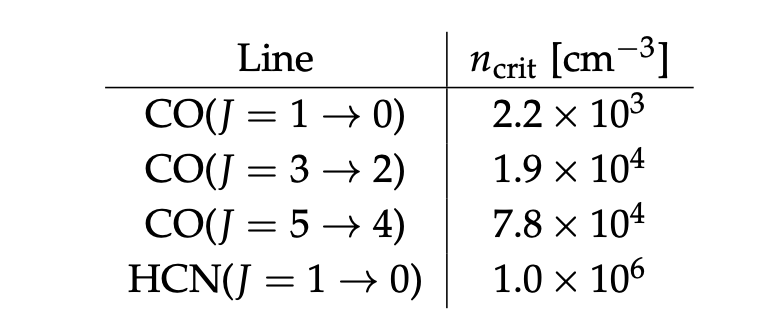
\includegraphics[width=6cm]{./figures/critical_density.png}
\end{center}
How do we interpret this though? A smaller critical density means a more diffuse region of $H_{2}$ is able to maintain a collisional de-excitation equal to the spontaneous emission of the molecule. It would then make sense that the lowest energy transition would require the lowest critical density.
\end{proof}

\noindent\textbf{(d).} Consider a molecular cloud in which the volume-averaged density is $n=100 cm^{-3}$. Assuming the cloud has a lognormal density distribution as given by the equation: 
\begin{equation}
p(s) = \frac{1}{\sqrt{2\pi\sigma_{s}^2}}exp\bigg[-\frac{(s-s_{0})^2}{2\sigma_{s}^2}\bigg]
\end{equation}
with a dispersion of $\sigma_{s}^2 = 5.0$, compute the fraction of the cloud mass that is denser than the critical density for each of these transitions. Which transtions are good tracers of the bulk of the mass in a cloud? Which are are good tracers of the denser, and thus more actively star-forming parts of the cloud?

\begin{problem}{1.2}
\textbf{Infrared Luminosity as a Star Formation Rate Tracer.}
We use a variety of indirect indicators to measure the star formation rate in galaxies, and one of the most common is to measure the galaxy's infrared luminosity. The underlying assumptions behind this method are that (1) most of the total radiant output in the galaxy comes from young, recently formed stars, and (2) that in a sufficiently dusty galaxy most of the starlight will be absorbed by dust grains within the galaxy and then re-radiated in the infrared. Explore this conversion works using the stellar population synthesis package Starburst99 (Leitherer et al., 1999; Vazquez \& Leitherer, 2005), http://www.stsci.edu/science/starburst99/.
\end{problem}

\noindent\textbf{(a).}
Consider the total luminosity of a stellar population in which star formation occurs at a fixed rate $\dot{M_{\star}}$. What is the expected relative ratio of $L_{tot}/\dot{M_{\star}}$ after 10Mry? After 100Myr? 1Gyr?
\begin{proof}[Solution]
Would expect that the star formation rate would decrease (meaning less stars created in each time step). In addition, the most massive (aka the most luminous stars) will have mostly died out after 100Myr so the total luminosity is also expected to decrease over time. So our ratio would decrease as the system ages.
\end{proof}

\noindent\textbf{(c).}
Try making the IMF slightly top heavy by removing all stars below $0.5M_{\odot}$. How much does the luminosity change for a fixed star formation rate? What do you infer from this about how sensitive this technique is to assumptions about the form of the IMF?
\begin{proof}[Solution]
By removing all of the low mass stars will obviously effect the overall luminosity of the star cluster, but since the vast majority of the luminosity is due to the few highest mass stars, the total effect will be muted. 
\end{proof}

\begin{problem}{2.1}
\textbf{The Bonnor-Ebert Sphere.}
Here we will investigate the properties of hydrostatic spheres of gas supported by thermal pressure. These are reasonable models for thermally-supported molecular cloud cores. Consider an isothermal, spherically-symmetric cloud of gas with mass M and sound speed $c_{s}$, confined by some external pressure $P_{s}$ on its surface.
\end{problem}

\noindent\textbf{(a).}
For the moment, assume that the gas density inside the sphere is uniform. Use the virial theorem to derive a relationship between $P_{s}$ and the cloud radius R. Show that there is a maximum surface pressure $P_{s,max}$ for which virial equilibrium is possible, and derive its value.
\begin{proof}[Solution]
The virial theorem requires:
\begin{equation}
0 = 2(T - T_{s}) + W
\end{equation}
With 
\begin{align}
W = \frac{-3}{5}\frac{GM^2}{R}, \\
T = \frac{3}{2}Mc_{s}^2, \\
T_{s} = 4\pi R^3 P_{s}
\end{align}
Let's now plug in everything into the virial equation, and solve for the external pressure $P_{s}$.

\begin{equation}
P_{s} = \frac{3Mc_{s}^2}{8\pi}\bigg[\frac{1}{R^3} - \bigg(\frac{GM}{5c_{s}^2}\bigg)\frac{1}{R^4}\bigg]
\end{equation}
What is obvious here, is that there are two terms: the first positive one dominates at large R, the second negative one dominates at small R. This means that there must be an intermediate maximum between these two extremes. So, determine this maximum, take the derivative of this equation and set equal to zero, solve for $R_{max}$ to obtain the location at which the maximum occurs. We can then solve for $P_{s}(R_{max})$. 
\end{proof}
\noindent\textbf{(b).}
We now consider the true density structure. Consider first the equation of hydrostatic balance:
\begin{align}
-\frac{1}{\rho}\frac{d}{dr}P = \frac{d}{dr}\phi
\label{eq:11}
\end{align}
Where $P=\rho c_{s}^2$ is the pressure and $\phi$ is the gravitational potential. Let $\rho_{c}$ be the density at $r=0$, and choose a gauge such that $\phi = 0$ at $r=0$. Integrate the equation of hydrostatic balance to obtain an expression relating $\rho, \rho_{c}, and \phi$.

\begin{proof}[Solution]
We can substitute in the given value of $P$ since the gas being described can be approximated to be isothermal. Then, plugging into \eqref{eq:11}, and using the trick that I simply must recall from Statistical Mechanics with Dr. Yuan: $\frac{1}{\rho}\frac{d}{d\rho} = \frac{d}{dr} ln(\rho)$. This trick makes this much easier to integrate: $-c_{s}^2 ln(\rho) = \phi + const$ and solving for density is also simple: 
\begin{equation}
\rho = \rho_{0}e^{-\phi / c_{s}^2}
\end{equation}
\end{proof}

\noindent\textbf{(g).}
The existance of a finite mass $m$ (average atomic mass) implies that, for a given dimensional mass $M$, there is a maximum surface pressure $P_{s}$ at which a cloud of that mass can be in hydrostatic equilibrium. Solve for this maximum and compare your result to the result obtained in part (a).
\noindent\textbf{(h.)}
Conversely, for a given surface pressure $P_{s}$ and sound speed $c_{s}$ there exists a maximum mass at which the cloud can be in hydrostatic equilibrium called the Bonnor-Ebert mass $M_{BE}$.
\begin{proof}[Explanation]
So, this is simply two different ways to describe the hydrostatic condition. The Bonnor-Ebert mass is most closely related to the Jean's instability condition, dealing with an isothermal sphere. 
\begin{align}
M_{BE} = m_{max}\frac{c_{s}^4}{P_{s}^{1/2}G^{3/2}}
\end{align}
\end{proof}

\begin{problem}{2.2}
\textbf{Driving Turbulence with Protostellar Outflows.}
Consider a collapsing protostellar core that delivers mass to an accretion disk at its center at a constant rate $\dot{M}_{d}$. A fraction $f$ of the mass that reaches the disk is ejected in to an outflow, and the remainder goes onto a protostar at the center of the disk. The material ejected into the outflow is launched at a velocity equal to the escape speed from the stellar surface. The protostar has a constant radius $R_{\star}$ as it grows. Ultimately, we want to know about protostellar outflows and their effects on star formation and star growth. 
\end{problem}

\begin{problem}{3.2}
\textbf{The Origin of Brown Dwarfs}
For the purposes of this problem, we will define a brown dwarf as any object whose mass is below $M_{BD} = 0.075 M_{\odot}$, the hydrogen burning limit. We would like to know if these could plausibly be produced via turbulent fragmentation, as appears to be the case for stars.

I'm guessing this is referring to the possibility that brown dwarfs condense straight out of turbulent gas as opposed to perhaps binary formation from gas bound to a more massive star?
\end{problem}
\noindent\textbf{(a).}
For a Chabrier (2005) IMF (see Chapter 2, equation 2.3), compute the fraction $f_{BD}$ of the total mass of stars produced that are brown dwarfs.
\begin{proof}[]

Equation 2.3 from Krumholz text depicts Chabrier Initial Mass Function:
\newline
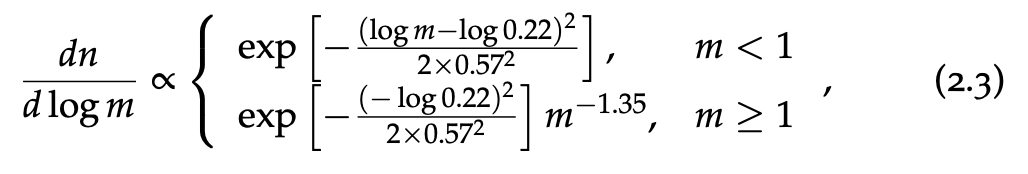
\includegraphics[width=8cm]{./figures/Chabrier05.png}
\newline
Computing the fraction of mass contained in brown dwarfs (less than 0.075 solar masses) we simply need to integrate the IMF across the mass range below the hydrogen burning limit and divide that by the total integrated mass greater than the burning limit. Easier said than done. We are going to need to do some coding for this one: Problem 3.2.ipynb
\begin{align}
f_{BD} = \frac{\int_{m_{min}}^{m_{BD}} \xi(m) dm}{\int_{m_{BD}}^{m_{max}} \xi(m) dm}
\end{align}
\end{proof}

\noindent\textbf{(b).}
In order to collapse, the brown dwarf must exceed the Bonnor-Ebert mass. Consider a molecular cloud of temperature 10K. Computer the minimum ambient density $n_{min}$ that a region of the cloud must have in order for the thermal pressure to be such that the Bonnor-Ebert mass is less than the brown dwarf mass.
\begin{proof}
The Bonnor-Ebert mass is defined as
\begin{align}
M_{BE} = 1.18 \frac{c_{s}^4}{\sqrt{G^3 P}} = 1.18 \frac{c_{s}^3}{\sqrt{G^3 \rho}}
\end{align}
Using $P = \rho c_{s}^2$. Solving for the density term $\rho$:
\begin{align}
\rho = \frac{(1.18c_{s}^3)^2}{G^3 M_{BE}^2}
\end{align}

Evaluating the density for a gas with $\mu = 2.3$ we can calculate the sound speed $c_{s}=\sqrt{k_{B}T/\mu m_{H}}=0.19$ km/s and so $\rho=9.3 \times 10^{-18}$ g cm$^{-3}$. And so, the number density can be simply calculated with $\rho/\mu m_{H} = n_{min} = 2.4\times10^6$ molecules/cm$^{-3}$.

\noindent\textbf{(c).}
Assume the cloud has a lognormal density distribution; the mean density is $\bar{n}$ and the Mach number is $M$. Plot a curve in the ($\bar{n}$, $M$) plane along which the fraction of the mass at densities above $n_{min}$ is equal to $f_{BD}$. Does the gas cloud that formed the cluster IC 348 ($\bar{n} \approx 5\times10^4$ cm$^{-3}$, $M \approx 7$) fall into the part of the plot where the mass fraction is below or above $f_{BD}$. 




\end{proof}

\begin{problem}{5.1}
\textbf{HII Region Trapping}
Consider a star of radius R$_{*}$ and mass M$_{*}$ with ionizing luminosity of S photons s$^{-1}$ at the center of a spherical molecular cloud. Assume the ionized gas has a sound speed of $c_{i} = 10$ km s$^{-1}$ and case B recombination coefficient of $\alpha_{B} = 2.6 \times 10^{-13}$ cm$^3$ s$^{-1}$.
\end{problem}
\noindent\textbf{(a).}
Suppose the cloud is accreting onto the star at a constant rate $\dot{M}_{*}$. The incoming gas arrives at the free-fall velocity, and the accretion flow is spherical. Compute the equilibrium ratios of the ionized region, and show that there is a critical value of $\dot{M}_{*}$ below which $r_{i} \gg R_{*}$. Estimate this value for $M_{*} = 30 M_{\odot}$ and S = 10$^{49}$ s$^{-1}$. How does this compare to typical accretion rates of massive stars?

\textit{EXPLANATION: The physicality of this problem is as follows: it is assumed that massive stars do not form directly from a cloud in a single event. Instead, the star will form and then accrete a significant amount of its final mass from the molecular cloud core. But, there are forces opposing the inward fall of the material to be accreted. The mechanism mentioned here is ionizing radiation. When the infalling hydrogen is ionized, its sound speed increases by a factor of 10, meaning its molecular speed at thermal equilibrium is not 10x higher. This may allow the material to escape the gravitational influence of the star.}
\begin{proof}
\textit{In this problem, we assume that the ionized region is stable, in equilibrium. This means that as gas continues to infall, the point at which it becomes ionized is unmoving. \textbf{This requires that the ionization rate and recombination rate in the region between the star and ionization front MUST be equal.}}

To begin, let's determine what the ionization rate per unit volume is:
\begin{align}
\alpha_{B}n_{e}n_{p} = 1.1\alpha_{B}(\rho / \mu_{H} m_{H})^2
\end{align}
So to describe the ionization rate per unit volume, we obviously need to describe the density of the gas being ionized. The gas to be ionized is the accretion flow. So, the density profile of the accretion flow is simply:
\begin{align}
\dot{M_{*}} = 4\pi r^2 \rho v_{ff}
\end{align}

Where $v_{ff} = \sqrt{2GM_{*}/r}$. Substituting into (18) and rearranging:
\begin{align}
\rho = \frac{\dot{M}_{*}}{4\pi \sqrt{2GM_{*}}}r^{-3/2}
\end{align}

So we can now plug in the density profile of the accretion flow to the recombination rate. This will tell us how the accretion flow reacts to the ionizing radiation. But, we ultimately want to describe the total recombination rate within the volume around the star that is beyond the stellar radius and within the ionizing front. So, let's perform that integral (integrate across a spherical area within the defined radius range):

\begin{align}
\Gamma = \int^{r_{i}}_{R_{*}} 4\pi r^2 (1.1\alpha_{B})\bigg(\frac{\dot{M}_{*}}{4\pi \mu_{H}m_{H}\sqrt{2GM_{*}}}r^{-3/2}\bigg)^2 dr \\
	= \frac{1.1\alpha_{B}\dot{M_{*}^2}}{8\pi\mu_{H}^2 m_{H}^2 GM_{*}}ln\frac{r_{i}}{R_{*}}
\end{align} 

Now, we can assert the condition described previously: ionization rate is equal to recombination rate (S = $\Gamma$). And we can then solve for the ionization front location $r_{i}$:

\begin{align}
r_{i} = R_{*}exp\bigg(\frac{8\pi\mu_{H}^2 m_{H}^2 GM_{*}S}{1.1\alpha_{B}\dot{M_{*}}}\bigg)
\end{align}

Now, we can easily determine the condition when $r_{i} \gg R_{*}$ is satisfied. It is when the exponent (term in parentheses) in eq (22) is greater than 1. Asserting this:

\begin{align}
\dot{M_{*}} \leq \Bigg(\frac{8\pi\mu_{H}^2 m_{H}^2 GM_{*}S}{1.1\alpha{B}}\Bigg)^{1/2}
\end{align}
So can the plug in the given values $M_{*} = 30M_{\odot}$ and S = $10^{49}$s$^{-1}$, we obtain $\dot{M_{*}} \leq 7 \times 10^{-5} M_{\odot}$ yr$^{-1}$.

\end{proof}

\noindent\textbf{(b).}
The H $II$ region will remain trapped by the accretion flow as long as the ionized gas sound speed is less than the escape velocity at the edge of the ionized region. What accretion rate is required to guarantee this? Again, estimate this numerically for the values given above.
\begin{proof}
The escape velocity at some distance $r$ from the star is $v_{esc} = \sqrt{GM_{*}/r}$. So, the condition that this value is less than the ionized sound speed leaves us with:
\begin{align}
\frac{2GM_{*}}{c_{i}^2} < r_{i} = R_{*}exp\bigg(\frac{8\pi\mu_{H}^2 m_{H}^2 GM_{*}S}{1.1\alpha_{B}\dot{M_{*}}}\bigg)
\end{align}
Solving for $\dot{M_{*}}$, the accretion rate onto the star,

\begin{align}
\dot{M_{*}} > \Bigg[\frac{8\pi\mu_{H}^2 m_{H}^2GM_{*}S}{2.2\alpha_{B}ln(v_{esc,*}/c_{i})} \Bigg]^{1/2}
\end{align}
Where we have used $v_{esc} = \sqrt{GM_{*}/R_{*}}$, since we are curious about the condition that traps the ionization front, forcing the gas to be accreted onto the stellar surface. Using R$_{*}$ = 7.7 R$_{\odot}$ (the radius of a 30 M$_{\odot}$ ZAMS star) and plugging in the other input values gives $\dot{M_{*}} > 2.2 \times 10^{-5} M_{\odot}$.

\end{proof}

\begin{problem}{5.2}
\textbf{The Transition to Grain-Mediated H$_{2}$ Formation.}
We will make rough estimates for how the Universe transitions from H$_{2}$ formation being mostly by gas-phase processes, as it must in the early universe where there are no metals, to H$_{2}$ formation being mostly on grain surfaces. 
\end{problem}
\noindent\textbf{(a).}
\begin{proof}

\end{proof}


\end{document}